%!TEX root =  main.tex
\section{Appendix: Parameter Selection}
\label{Sec:AppOptPars}

Empirical results guiding parameter selection are presented on the following
pages in Figure~\ref{fig:par-plot-1} ($\epsilon$ = .1) and Figure~\ref{fig:par-plot-2} 
($\epsilon$ = 1). 

\begin{figure*}[h]
\centering
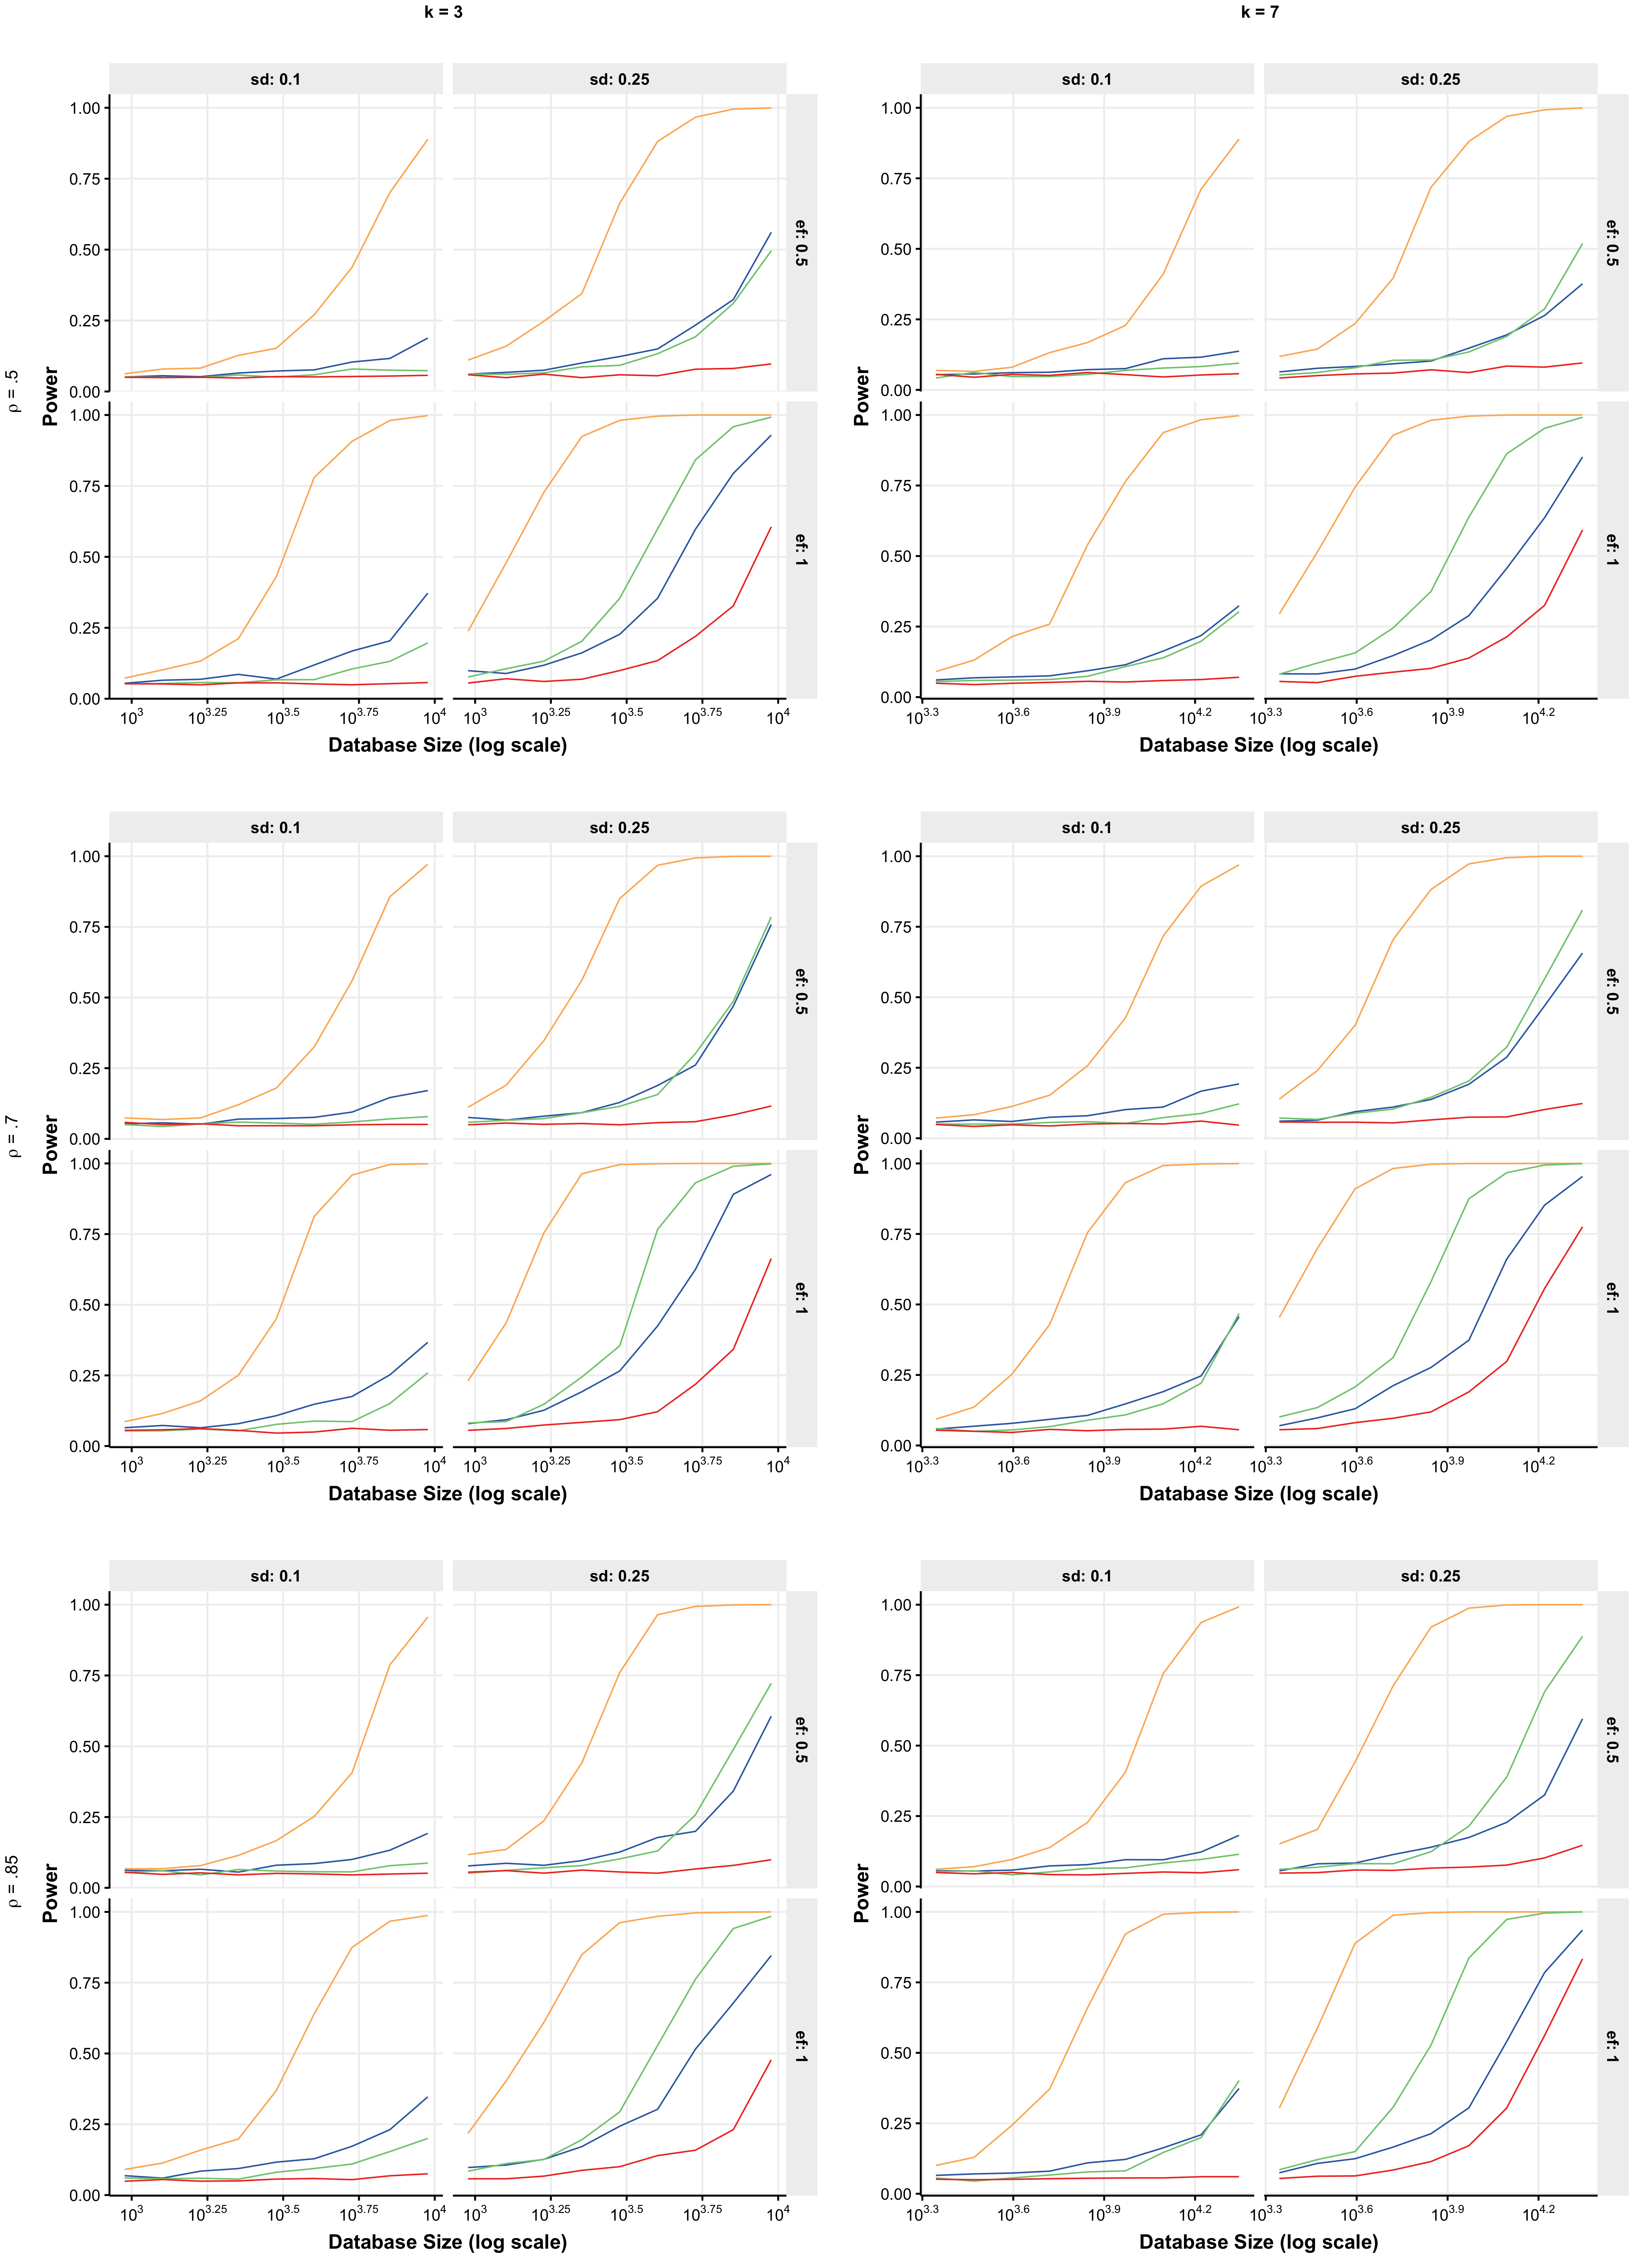
\includegraphics[width=\linewidth]{par-plot-1.png}
\caption{Power comparison in settings where $\epsilon = .1$. Within each subplot,
each color curve corresponds to a different value of $q$ (blue: 0.75, gold: 1,
green: 1.5, red: 2). The two main columns
of plots correspond to different values of $k$ and the three main rows correspond
to difference values of $\rho$. Note that the scale on the x-axis differs with $k$
($k = 7$ requires more data).}\label{fig:par-plot-1}
\end{figure*}

\begin{figure*}[h]
\centering
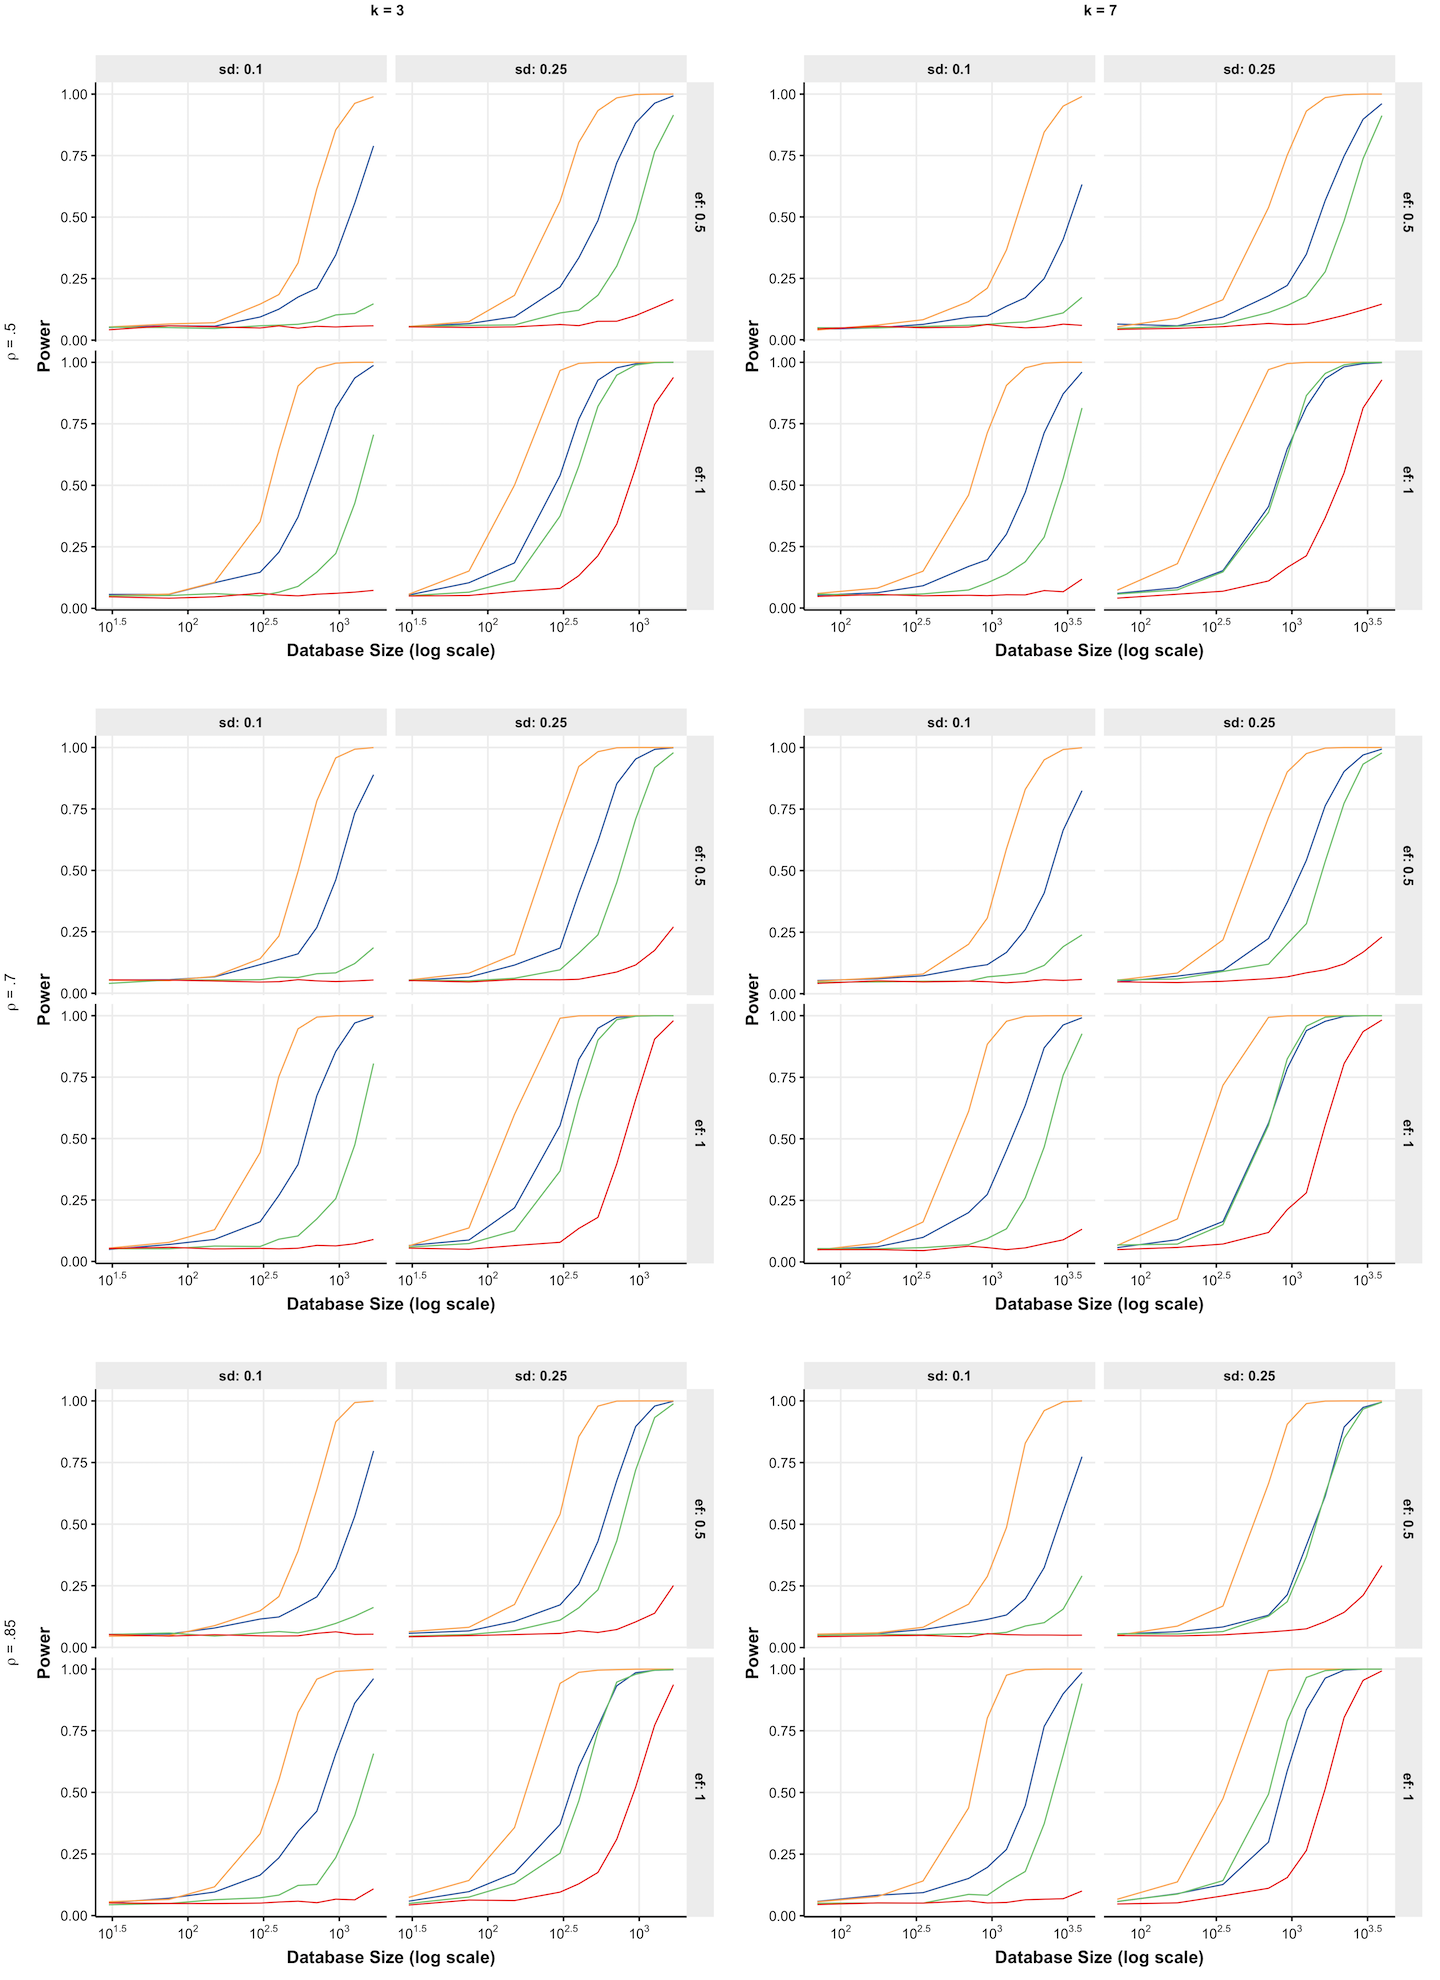
\includegraphics[width=\linewidth]{par-plot-2.png}
\caption{Power comparison in settings where $\epsilon = 1$. Within each subplot,
each color curve corresponds to a different value of $q$ (blue: 0.75, gold: 1,
green: 1.5, red: 2). The two main columns
of plots correspond to different values of $k$ and the three main rows correspond
to difference values of $\rho$. Note that the scale on the x-axis differs with $k$
($k = 7$ requires more data).}\label{fig:par-plot-2}
\end{figure*}
